% Chapter 4
%
\chapter{In-depth Design of SendIt} % Main chapter title
%
%4. Specific design
	%Serverless
		%Use Case
		%Program Flow
		%Specific implementation (of technology)

	%Assisted connection setup
		%Use Case
		%Program Flow
		%Specific implementation (of technology)

\label{Chapter4} % For referencing the chapter elsewhere, use \ref{Chapter1} 
%
In this chapter the in-depth design and functionality of SendIt will be discussed. The program flow and use of the application will be illustrated and the two different modes will be contrasted and compared.

SendIt consists of two modes: Serverless and Assisted Connection Setup (ACS). The difference between these modes is how the setup of the connection is completed, as illustrated in \Cref{fig:mode_comparison}. This affects the flow of the program and also impacts how easy it is to use. In the following sections the differences will be clearly shown and suggestions on how to best utilize the system will be given. It is important to note that neither mode changes the required technical knowledge to use the program - only the interactions required. This is to make sure all users can utilize both modes.

%
\begin{figure}
	\centering
	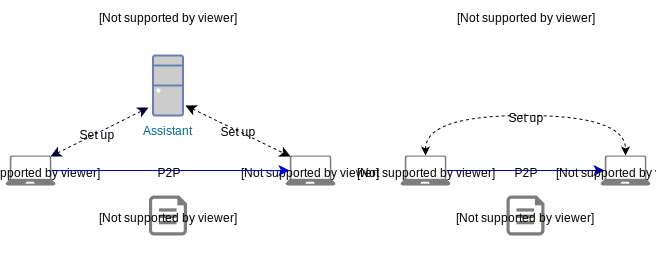
\includegraphics[width=\textwidth]{Figures/SendIt_mode_comparison}
	\caption[SendIt mode comparison]{Left: Assisted Connection Setup mode, Right: Serverless mode} \label{fig:mode_comparison}
\end{figure}

%
\section{Serverless mode}
%
Serverless mode is a mode completely independent of servers (as the name indicates) when establishing the connection. This mode allows the users to be unpredictable in how the offer/answer exchange is done and maximizes the improved security of SendIt. It does however slightly lower the ease of use and requires more from the end user.
%
\subsection{Use case}
%
As indicated above, the use case for this mode is by and large for those who values security over usability. This mode should be used if you are already having a conversation with the other endpoint and can quickly take care of the connection setup. Say Alice is talking to Bob and wants to transfer a file. Alice and Bob then take care of the connection setup using an instant messaging service. This allows for a quick and easy file-transfer, while getting the added bonus of having the file transferred in a very secure manner. Another example is if Bob wants to transfer an extremely sensitive file to Alice. They can then make a plan on what time they are to do the transfer, to be able to take care of the connection setup quickly. This way the file transfer is done with the highest level of security achievable in the system.

As illustrated above, at the cost of some of the usability this mode gives full control to the end user as to how the sharing of the offer/answer is done. It does require more manual interactions as well as more planning. This is because the lifetime of the offer/answer exchange puts a time limit on the exchange. It is also because the user has to manually transfer the part generated by their own application and manually input the part received from the other endpoint. There is no change in the technical knowledge requirements to use this mode, just the time constraint and manual interactions as mentioned above.
%
\subsection{Program flow}
%
The program flow is explained from the home screen. For information about functionality other than Send and Receive, see the explanation in \Cref{sec:progflow}.
The program flow of the serverless mode varies depending on if the user is taking the role of sender or receiver. As such, the next part will take you through the two different roles, the choices and screens showed, as well as what is going on. If the user has not chosen an identity yet, this screen will always be the first to appear, after choosing the intended functionality (\emph{Send/Receive}):
\begin{figure}[H]
  \centering
  \includegraphics[width=\textwidth]{Figures/SL/pop_up_own}
  \decoRule
  \caption[Enter own e-mail address screen]{A pop up forcing the user to choose which identity (e-mail) to use}
  \label{fig:serv_popown}
\end{figure}

%If user not stored, username required!

\subsubsection*{Sender:}
%
\noindent
\underline{First screen}
\begin{figure}[H]
  \centering
  \includegraphics[width=\textwidth]{Figures/SL/send_pop_up}
  \decoRule
  \caption[Enter recipient screen]{A pop up forcing the user to input the recipients identity (e-mail)}
  \label{fig:serv_s_pop}
\end{figure}
%1.1 Input recipients email
%	Required for encryption and authentication

%
\noindent
\underline{Second screen}\\
On this screen, an empty white box appears. Once the offer is ready, it will appear in the box along with a notification informing the user that it has been copied to the clipboard automatically. The offer can either be in cleartext or encrypted. Underneath, there is data about which file(s) are to be transferred. It also indicated the file in red, if it is not included in the transfer. Finally, there is a continue button that is only clickable after the offer has been shown.
\begin{figure}[H]
  \centering
  \includegraphics[width=\textwidth]{Figures/SL/offer}
  \decoRule
  \caption[Offer screen]{This screen displays the offer and the file(s) to be shared. The user should share this offer with the intended recipient.}
  \label{fig:serv_s_off}
\end{figure}
	%1.2 send screen - show offer details, files to send \& recipient
	%-> Share with other user
	%	Displays the files ready for transfer: Name, type, size. After a short delay, the offer will appear in the box. Either encrypted (if previous communication has happened.) or in cleartext (If first time communicating). This is automatically copied to clipboard. Press continue once offer has been shared.

%
\noindent
\underline{Third screen}
\begin{figure}[H]
  \centering
  \includegraphics[width=\textwidth]{Figures/SL/sender_answer}
  \decoRule
  \caption[Input answer screen]{This screen displays another white box where the user should paste the answer received from the Recipient. The continue button is only clickable after some information has been entered into the box.}
  \label{fig:serv_s_ans}
\end{figure}
%2 Answer screen - input answer
%		Displays a box where the user should paste the answer received from the other endpoint. Once done, click the continue button
	%

\subsubsection*{Receiver:}

%
\noindent
\underline{First screen}
\begin{figure}[H]
  \centering
  \includegraphics[width=\textwidth]{Figures/SL/receiver_pop_up}
  \decoRule
  \caption[Enter Sender screen]{A pop up forcing the user to input the Senders identity (e-mail)}
  \label{fig:serv_r_pop}
\end{figure}

%
\noindent
\underline{Second screen}
\begin{figure}[H]
  \centering
  \includegraphics[width=\textwidth]{Figures/SL/receiver_offer}
  \decoRule
  \caption[Enter offer screen]{This screen displays a white box where the user should paste the offer received from the Sender. The continue button is only clickable after some information has been entered into the box.}
  \label{fig:serv_r_off}
\end{figure}
%	1. Input offer \& senders mail
%		Box for pasting offer and indicating who the sender is, for correct encryption and authentication. Click continue once the offer is pasted. (Offer can be cleartext or cipher!)

%
\noindent
\underline{Third screen}
\begin{figure}[H]
  \centering
  \includegraphics[width=\textwidth]{Figures/SL/answer}
  \decoRule
  \caption[Answer screen]{This screen displays an empty white box, until the answer is generated. Once it is generated, it appears in the box along with a notification that it has been copied to the clipboard. The user should share this answer with the Sender.}
  \label{fig:serv_r_ans}
\end{figure}
%	2. Show answer
%		Shows box for displaying the answer. After a short wait, the answer will appear in the box, as well as automatically be copied to the clipboard. This can be either encrypted or cleartext, depending on if it is the first time communicating or not.

\subsubsection*{Shared:}
After the steps above, the functionality and screens are the same for both the Sender and the Recipient. They are as indicated below.\\
\\
%
\noindent
\underline{Fourth screen}
\begin{figure}[H]
  \centering
  \includegraphics[width=\textwidth]{Figures/SL/waiting}
  \decoRule
  \caption[Waiting screen]{This screen is displayed while waiting for the endpoints to connecting via P2P. (WebRTC)}
  \label{fig:SL_wait}
\end{figure}

%
\noindent
\underline{Fifth screen}\\
	It displays details about the current file being transferred, its name, size and type as well as total number of files to transfer. It also shows the \% of data transferred for the current file. Finally, there is a cancel button in case one end wants to stop the transfer.
\begin{figure}[H]
  \centering
  \includegraphics[width=\textwidth]{Figures/SL/transfer}
  \decoRule
  \caption[Transfer screen]{Details about the transfer displayed. }
  \label{fig:SL_trans}
\end{figure}

%
\noindent
\underline{Sixth screen (\emph{Sender})}
\begin{figure}[H]
  \centering
  \includegraphics[width=\textwidth]{Figures/SL/sender_complete}
  \decoRule
  \caption[Final screen Sender]{Shows details about which files were transferred.}
  \label{fig:SL_rec1}
\end{figure}

%
\noindent
\underline{Sixth screen (\emph{Receiver})}
\begin{figure}[H]
  \centering
  \includegraphics[width=\textwidth]{Figures/SL/receiver_complete}
  \decoRule
  \caption[Final screen Receiver]{Shows details about which files were transferred. Also has an 'open in folder'-button for easy access to the received files.}
  \label{fig:SL_rec2}
\end{figure}

\subsection{Implementation specifics}
%
The biggest difference in implementation, is of course the connection setup. Since it is non-existent in the serverless solution, the additional features will be discussed in \Cref{sec:acsimp}. In serverless mode, the offer and answer is displayed in the form of a string. The string can either represent a cipher or a cleartext representation of the offer/answer.

Since this part of SendIt has user interactions and rely on converting user input into JavaScript objects, it was at risk for XSS attacks or other code execution attacks. As such input sanitation was added to make sure that such attacks can not be executed. All data, both exported and imported in this phase has to conform to the JSON format, which is then parsed and turned into JavaScript Objects and used for establishing the connection via WebRTC.
%
\subsection{Possible improvements \& extendability}
%
This mode allows for no server-involvement, which in itself is a great way to reduce expenses. For SendIt it is only applied to file transfers, and datachannels. If this is applied to VOIP, which is currently one of the the most used application of WebRTC, it could allow companies to increase profit margins. This does however, set requirements for improving the lifetime of the connection setup. Especially the answer needs to have its lifetime doubled or tripled for it to be likely to be usable in this scenario.

If one can somehow make changes to the current WebRTC system and makes endpoints permanently addressable by a specific offer/answer, or allow the offer/answer to be re-usable, it would also benefit this solution a lot. Of course these permanent addressing or reusable offers/answers would have to be unique for each pairing, which might also raise some new issues. Working on extending the lifetime of the connection setup is objectively the best and most effective way to improve this solution.
%
%
\section{Assisted Connection Setup mode \textbf(ACS)}
%
%TODO REVIEW
Assisted connection setup mode alleviates some of the difficulties and problems from the serverless mode, by automatically taking care of the connection setup. This is done through a server, communicating by WS over HTTPS. It uses a custom protocol on top of WS, designed for sharing connection information for WebRTC, to control and understand the communication between the endpoints.

The server can be explicitly chosen by the users. They can host their own or choosing from an existing one offering this service. The only requirement is adhering to the pre-configured protocol. For details about the protocol, see \Cref{sec:wsprot} Because of this, the system is still unpredictable and hard to attack.

There is no need for the server to send code to be executed or loaded by the client, as this functionality is preprogrammed in the client application. As such the server has \emph{no} influence over the functionality of the client. The server only authenticates the user, and forwards the connection information to the other endpoint.
In addition, all communication with the ACS happens over a secure channel, so an attacker would have to break the server itself to gain access to the information relayed. For more information about how the ACS server and the client communicates, see \Cref{sec:acsws}
%
\subsection{Use case}
%
%TODO REREAD
The use case for this mode is when planning or co-ordinating with the other endpoint is not done in advance or hard to do. It is for when one is willing to sacrifice a small degree of security to improve the usability. This mode allows for the request to be sent, but the connection setup is not done until the other endpoint has agreed to take part in the exchange. As such the lifetime of the offer/answer is not an issue, since the exchange does not happen until both endpoints are online and ready to exchange information. It happens through an intermediary, so the exchange is almost instant. Since this intermediary is a point of attack and monitoring, it adds a small weakness to the system compared to the serverless mode.
%
\subsection{Program flow}
%
The program flow is explained from the home screen. For information about functionality other than Send and Receive, see the explanation in \Cref{sec:progflow}.
The ACS mode program flow differs depending on if the user has the role of sender or receiver. As such, the program flow of both of the roles will be shown and explained below.

Both roles begin with this screen, when entering ACS mode (This can be when starting the application, or when switching modes):
%
\begin{figure}[H]
  \centering
  \includegraphics[width=\textwidth]{Figures/ACS/pop_up}
  \decoRule
  \caption[Opening screen]{The ACS mode requires an identity to be given, in order to be able to authenticate with the ACS server. This is also done so the ACS server knows where to forward data for each identity.}
  \label{fig:ACS_pop}
\end{figure}

\subsubsection*{Sender:}
%
\noindent
\underline{First screen}
\begin{figure}[H]
  \centering
  \includegraphics[width=\textwidth]{Figures/ACS/sending}
  \decoRule
  \caption[Sending details screen]{This screen displays the e-mail for the current identity, a field to indicate the Receivers e-mail and information about the file(s) to be transferred. If a file is marked in red, it means it will not be included.}
  \label{fig:ACS_send}
\end{figure}

\subsubsection*{Receiver:}
%
\noindent
\underline{First screen}\\
	It displays the e-mail for the current identity, the e-mail of the intended receiver (as indicated by the Sender), the Senders e-mail, and data about the file(s). The user has two buttons: Accept and Decline. If the decline button is pressed, the user returns to the home screen.
\begin{figure}[H]
	\centering
	\includegraphics[width=\textwidth]{Figures/ACS/receiving}
	\decoRule
	\caption[Connection request screen]{This screen notifies the user that another user wants to share a file.}
  \label{fig:ACS_rec}
\end{figure}
%
\subsubsection*{Shared:}
After the steps above, the functionality and screens are the same for both the Sender and the Recipient. They are as indicated below.\\
\\
%
\noindent
\underline{Second screen}
\begin{figure}[H]
  \centering
  \includegraphics[width=\textwidth]{Figures/ACS/waiting}
  \decoRule
  \caption[Waiting screen]{This screen is displayed while waiting for the endpoints to connecting via P2P. (WebRTC)}
  \label{fig:ACS_wait}
\end{figure}

%
\noindent
\underline{Third screen}\\
	It displays details about the current file being transferred, its name, size and type as well as total number of files to transfer. It also shows the \% of data transferred for the current file. Finally, there is a cancel button in case one end wants to stop the transfer.
\begin{figure}[H]
  \centering
  \includegraphics[width=\textwidth]{Figures/ACS/transfer}
  \decoRule
  \caption[Transfer screen]{Details about the transfer displayed. }
  \label{fig:ACS_trans}
\end{figure}

%
\noindent
\underline{Fourth screen (\emph{Sender})}
\begin{figure}[H]
  \centering
  \includegraphics[width=\textwidth]{Figures/ACS/sender_complete}
  \decoRule
  \caption[Final screen Sender]{Shows details about which files were transferred.}
  \label{fig:ACS_rec1}
\end{figure}

%
\noindent
\underline{Fourth screen (\emph{Receiver})}
\begin{figure}[H]
  \centering
  \includegraphics[width=\textwidth]{Figures/ACS/receiver_complete}
  \decoRule
  \caption[Final screen Receiver]{Shows details about which files were transferred. Also has an 'open in folder'-button for easy access to the received files.}
  \label{fig:ACS_rec2}
\end{figure}

%
\noindent
\underline{Fifth screen}
\begin{figure}[H]
  \centering
  \includegraphics[width=\textwidth]{Figures/ACS/error}
  \decoRule
  \caption[Error screen]{This screen shows where the error will appear. The message varies depending on which error occurs.}
  \label{fig:ACS_err}
\end{figure}

%
\subsection{Implementation specifics}
\label{sec:acsimp}
%
The biggest difference in implementation comes in the form of how the connection setup is exchanged and processed. Following, the way of communicating with the ACS server and how the WebRTC connection setup is done, will be explained. The functionality for actually sending the file(s) stays the same, but since the connection setup happens through a server, it needs a secure way to interact with the server. In this section the client-side implementation will be described. For more information about the server and the protocol used, please see \Cref{sec:acs_serv}. 
%
\subsubsection*{Communication:}
%TODO review
The ACS mode utilizes WebSockets to communicate with the server. It forces the use of HTTPS as well, to make sure that all communications is secure. All communication has to be in the format of the protocol described in \Cref{sec:wsprot}. This means that the information that is going to be shared has to be processed and then correctly represented. Based on the information exchanged with the endpoint via the ACS, a P2P connection is established, just like in the serverless mode. At this point the ACS server is no longer utilized. Once the connection has finished for whatever reason, the ACS server is notified that the connection is over and that the endpoint is ready for a new connection.
%
\subsubsection*{WebRTC Connection setup:}
There are two major changes in how the connection setup for the P2P channel changes in this mode. First of all, the exchange does not just happen in the form of one offer and one answer. The method called ICE trickling, as described in \Cref{sec:webrtc_icetri} is used. This separates the offer and answer from the ICE candidates. This allows for continuous exchange of ICE candidates, as well as a faster exchange of the offer and answer, since they can be shared without waiting for all the ICE candidates to be gathered before being shared. As such the lifetime of the offer and answer is irrelevant in this mode.

Secondly, the connection setup does not happen until both endpoints have agreed to connect to each other. This means that the endpoints are ready to receive and process the offer/answer and allows the exchange to happen almost instantaneously. This minimizes the risk of any issues arising when doing the exchange and allows for an efficient connection setup. It also means that the endpoints does not redundantly create an offer, wasting time, in the case that the other endpoint declines the connection.

Finally, the roles of sender and receiver in SendIt, compared to in WebRTC, is reversed. This is to avoid the redundant creation of an offer, as mentioned in the section above. The receiver in SendIt will receive a connection offer in the form of the screen showed in \Cref{fig:ACS_rec}. If the endpoint accepts this connection offer by pressing the accept-button, a WebRTC offer will be generated and exchanged via the ACS server. Afterwards, functionality will be the same as in serverless mode.
%
\subsection{Possible improvements \& extendability}
%
%REVIEW
Most of the improvements and extendability for this mode will rely on making changes to the current functionality of the ACS server. It would also require changes to the ACS client code, and as such, the discussion will be done in this section.

\subsubsection*{Key request:}
%Review
%REVIEW
Allowing the endpoints to request the key for an identity, via the ACS server, would allow for encrypted end-to-end communication at all times. This requires some guarantee from the owner of the key to be attached, so the ACS server can not easily set up a MitM-attack. This would remove some of the issues with trusting the first exchange, and also allow for better trust evaluation and improved key exchange. The difficulty arises in the fact that the information needs to have a guarantee that it belongs to the correct identity, without having any previous or additional communication. One way to achieve this functionality is to go through the additional channel of using e-mail as a means of exchanging some shared secret, but this is left up to future work.
%
\subsubsection*{Multicast:}
%Review
Extending SendIt to allow false multicast messages would mimic the way current e-mail attachments work and make sharing a file with multiple recipients at once easier. The reason for calling it false multicast, is because the transfer would still be one to one, but for the sender, it would seem identical to transferring to a single recipient. While this may allow for rapid spreading of malicious files, it would also improve usability by a lot, in in legitimate use cases. A way to achieve this is to have each client connect to a 'room' in the server, where the sender has to authenticate endpoints before/upon entering. After being authenticated, a P2P connection between the sender and the endpoint can be established and the file transferred.
%
\subsubsection*{Automatic reconnect:}
%Review
Automatically reconnecting after an endpoint has been disconnected or gone offline, would be a huge improvement to usability and user friendliness. It would allow for a very smooth user experience and increase the stability and reliability of the system. A way to achieve this would be to assign connections as broken, if one endpoint reports a broken connection to the ACS server. Once the ACS server detects that the endpoint is available again, it would automatically start the connection setup for both endpoints. The endpoints should have functionality that automatically accepts and connects, if this is the case.
%
\subsubsection*{Pausing connections:}
%Review
Allowing for pausing connections would increase user friendliness and help alleviate some issues that present when using synchronous communication. It would require some way to resume transfers from their previous point, but with such functionality in place, it should not be to hard to implement pausing connections. This would primarily be useful when being in the middle of a connection, when the need for transferring another file urgently occurs. Say the user is transferring a movie to a friend, when all of a sudden an important document from work needs to be received. Being able to temporarily pause the movie-transfer, receive the document, then resume the movie-transfer would be very useful. Having it automatically done through the ACS server, would be preferred.